\begin{frame}{Update rules}
    
    \begin{itemize}
        \item An update rule is a finite set $X\subseteq\mathbb{Z}^2-\{0\}$
        \item An update family is a finite collection of update rules $\mathcal{U}=\{X\subseteq\mathbb{Z}^2-\{0\}\}$
    \end{itemize}
    
 
\begin{block}{}
   
 $\mathcal{U}$-Bootstrap percolation initialized at $A$ refers to the following process:

 \begin{itemize}
     \item $A_0=A$
     \item $A_{t+1}=A_t\cup \{x\in\mathbb{Z}^2: x+X\subseteq A_t \textit{ for some } X\in\mathcal{U}\}$
 \end{itemize}
 \end{block}
 
 \end{frame}
 \begin{frame}

 \begin{itemize}
 
 
     \item The set $A$ is known as the set of initially infected sites
     \item The closure of $A$ is defined as $[A]=\cup_{t\geq 0} A_t$
     \item The initialization is random i.e. each site (vertex)
     in $\mathbb{Z}^2$ is infected with probability $p$ independently from the other vertices
     \item The process is monotone i.e. if a site gets infected, it stays infected forever
     \item After the initialization, the process is deterministic in the sense that a site will get infected if and only if there is some rule $X$ in $\mathcal{U}$ such that $x+X$ is infected
 \end{itemize}
 


\end{frame}




\begin{frame}{Examples}
\begin{figure}
  \centering
  \begin{subfigure}{.2\linewidth}
    \centering
    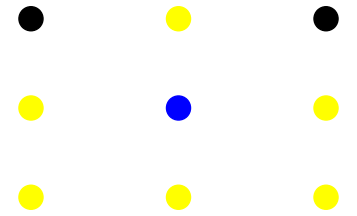
\includegraphics[width = \linewidth]{rgospercrule.png}
    \caption{Oriented site percolation}
  \end{subfigure}%
  \hspace{2em}% Space between image A and B
  \begin{subfigure}{.2\linewidth}
    \centering
    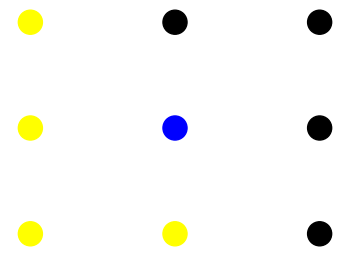
\includegraphics[width = \linewidth]{rgspiralpercrule1.png}
    \caption{$U_1$ for Spiral}
  \end{subfigure}%
  \hspace{2em}% Space between image B and C
  \begin{subfigure}{.2\linewidth}
    \centering
    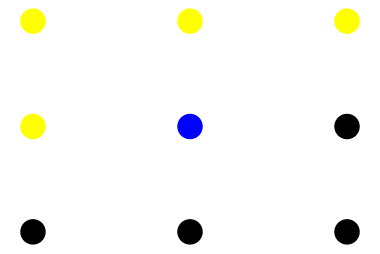
\includegraphics[width = \linewidth]{rgspiralpercrule2.png}
    \caption{$U_2$ for Spiral}
  \end{subfigure}
  	\label{fig:mesh1}
\end{figure}


\begin{itemize}
    \item r-Neighbour models for r=1,2,3,4
    \item Oriented site $\mathcal{U}=\{(-1,1),(1,1)\}$
    \item Spiral $\mathcal{U}=\{U_1,U_2,U_3,U_4\}$, where 
    $U_1=\{(1,-1),(1,0),(1,1),(0,1)\}$
    \newline
    $U_2=\{(1,-1),(1,0),(-1,-1),(0,-1)\}
    $
    \newline
    $ U_3=-U_1, U_4=-U_2$
    \item Directed triangular bootstrap percolation 
    

\end{itemize}



\end{frame}

\begin{frame}{Stable directions, basic properties}
For a vector $u\in\mathbb{S}^1$, we define $
\mathbb{H}_u=\{x\in\mathbb{Z}^2|<x,u><0\}$.

\begin{block}{Definition}



Given an update family $\mathcal{U}$, a direction $u\in\mathbb{S}^1$ is
\begin{itemize}

    \item stable if $[\mathbb{H}_u]=\mathbb{H}_u$. The set of stable directions is denoted by $\mathcal{S}=\mathcal{S}(\mathcal{U})$
    \item strongly stable if $u\in int\mathcal{S}$
    \item unstable if it is not stable


\end{itemize}
\end{block}


\begin{itemize}
    \item Dichotomy $[\mathbb{H}_u]\in\{\mathbb{H}_u,\mathbb{Z}^2\}$
    \item $\mathcal{S}\subseteq\mathbb{S}^1$ is a set of stable directions for some update familit $\mathcal{U}$ if and only if it can be expressed as a union of closed intervals with rational endpoints\footnote{A direction $u\in\mathbb{S}^1$ is said to be rational if there is a point in the grid $\mathbb{Z}^2\cap\{\lambda u|\lambda\in\mathbb{R}\}$
    1}
    in $\mathbb{S}^1$
\end{itemize}



\end{frame}

\begin{frame}{Classification of $\mathcal{U}$-Bootstrap percolation}
$\mathcal{U}$-bootstrap percolation update families exhibit different properties based on their stable sets. Let $\mathcal{U}$ be an update family with a set of stable directions $\mathcal{S}$
\begin{block}

\begin{itemize}
    \item If there is a open semicircle $C$ such that $\mathcal{S}\cap C=\emptyset$ then $\mathcal{U}$ is said to be \emph{supercritical}
    \item If every open semicircle $C$ intersects $\mathcal{S}$, but there is an open semicircle $C_0$ that doesn't intersect $int\mathcal{S}$ then $\mathcal{U}$ is said to be \emph{critical}
    \item If every open semicircle $C$ intersects $int S$ then $\mathcal{U}$ is said to be \emph{subcritical}
\end{itemize}

\end{block}

\end{frame}

\begin{frame}{Supercritical and critical families}
\begin{block}{Infection time of the origin}
The infection time of 0 is defined as $\tau_p=\inf\{t\in\mathbb{N}: 0 \in A_t\}$, given that $A_0=A$ is sampled according to a Bernoulli $p$ distribution
\end{block}

\begin{itemize}
    \item For supercritical families, $\tau_p=p^{-\Theta(1)}$ as $p\rightarrow 0$ with high probability
    \item For critical families, $\tau_p=\exp(p^{-\Theta(1)})$ as 
    $p\rightarrow 0$ with high probability
\end{itemize}

Corollary\footnote{\textsc{Bollobás, Smith, Uzzel}, Monotone Cellular automata in a random environment, \emph{Combinatorics, Probability and Computing}, 2015}: For supercritical and critical families, $p_c=\inf\{p>0|P_p([A]=\mathbb{Z}^2)=1\}=0$ i.e. for any $p>0$ we have percolation.

    
\end{frame}


\begin{frame}{Subcritical Families}

\begin{itemize}
    \item For subcritical families $p_c>0$\footnote{\textsc{Balister, Bollobás, Przykucki, Smith}, Subcritical $\mathcal{U}$-Bootstrap percolation models have non-trivial phase transitions, \emph{arXiv},2019}
    \item Percolation at $p=p_c$ is open
    \item Behaviour of $\tau_p$ as $p\rightarrow p_c$ from above is open
    \item Exponential decay answered 
    \item Infinite component without percolation answered
\end{itemize}
    
\end{frame}
